%%%%%%%%%%%%%%%%%%%%%%%%%%%%%%%%%%%%%%%%%%%%%%%%%%%%%%%%%%%%%%%%%%%%%%%%%%%%
%
%  Template code for the Undergraduate Research Scholars thesis program starting, updated by Undergraduate Research Scholars program staff. Version 6.0. Last Updated: Fall 2024
%  Modified by Tawfik Hussein from the template code for TAMU Theses and Dissertations starting Spring 2018, authored by Sean Zachary Roberson. Version 3.17.09.
%
%
%%%%%%%%%%%%%%%%%%%%%%%%%%%%%%%%%%%%%%%%%%%%%%%%%%%%%%%%%%%%%%%%%%%%%%%%%%%%%%%

%%%%%%%%%%%%%%%%%%%%%%%%%%%%%%%%%%%%%%%%%%%%%%%%%%%%%%%%%%%%%%%%%%%%%%%%%%%
%%                           APPENDIX 
%%%%%%%%%%%%%%%%%%%%%%%%%%%%%%%%%%%%%%%%%%%%%%%%%%%%%%%%%%%%%%%%%%%%%%%%%%%

% The Appendix section is optional, must be placed directly after the references section, can be a collection of large data sets, images, and/or tables tghat would interrupt a significant portion of your writing. It can be a single Appendix (label as Appendix: Title) or it can include multiple Appendices (label as Appendix A: Title, Appendix B: Title, etc). Label figures, tables, and equations consecutively starting with A.1, A.2, etc. For additional Appendices (B, C, etc.), label figures, tables, and equations as B.1, B.2, etc. It can also be as many pages as needed.

%_________(0)____________

% Do not modify this section. This ensures proper formatting of the appendix tables, equations, and figures.

\phantomsection

\chapter*{\large\bf APPENDIX A: SOURCE CODE}
\addcontentsline{toc}{chapter}{APPENDIX A: SOURCE CODE} 


%___________(1)____________
% Modifications needed! 

% [INSTRUCTIONS FOR REQUIRED ACKNOWLEDGEMENTS PAGE.]

%The Appendix section: 
%\begin{itemize}
%  \item Is optional
%  \item Must be placed directly after the References section
%  \item Can be a collection of large data sets, images, and/or tables that would interrupt a significant portion of your writing
%  \item Can be a single Appendix (label as Appendix: Title)
%  \item Can include multiple Appendices (label as Appendix A: Title, Appendix B: Title, etc.)
%  \item Label figures, tables, and equations consecutively starting with A.1, A.2, etc. For additional Appendices (B, C, etc.), label figures, tables, and equations as B.1, B.2, etc.
%  \item Can be as many pages as needed
%\end{itemize}

%____________(2)_________________
% MODIFY THE SAMPLE APPENDIX PAGE. INCLUDES EXAMPLE FIGURES WITH PROPER CAPTION LABELLING AND NUMBERING. 
\indent\indent This appendix contains links to our open-source implementations of the algorithms discussed in this paper. Detailed instructions for usage and experimentation can be found in the README files of the respective repositories.

\begin{itemize}
	\item \href{https://github.com/lilacstella/replicate\_alpha\_regex}{\textbf{Replicating AlphaRegex Algorithm}} \\
	Visit: \texttt{https://github.com/lilacstella/replicate\_alpha\_regex} \\
	A reimplementation of the AlphaRegex algorithm, featuring a greedy search over regex syntax trees guided by cost heuristics. Includes benchmark evaluation and custom weight tuning options.
	
	\item \href{https://github.com/lilacstella/replicate\_l\_star}{\textbf{Replicating L* Algorithm}} \\
	Visit: \texttt{https://github.com/lilacstella/replicate\_l\_star} \\
	An implementation of the L* learning algorithm that synthesizes DFAs from membership and equivalence queries, with conversion to regex via Brzozowski's method.
\end{itemize}



\chapter*{\large\bf APPENDIX B: EXAMPLE L* REGEX GENERATION}

\addcontentsline{toc}{chapter}{APPENDIX B: EXAMPLE L* REGEX GENERATION} 


\renewcommand{\thefigure}{B.\arabic{figure}}
\setcounter{figure}{0}

\indent\indent The following is the output of an example run of my implementation of the L* algorithm. The goal is to achieve the regex \texttt{.*ab.*}, but the algorithm yielded an equivalent regex. The L* application interacts with the MAT by continuously prompting for membership queries, DFA proposals, and counterexamples until the process is complete.

\lstset{
  basicstyle=\ttfamily,
  escapeinside={*@}{@*}  % allows LaTeX inside listings
}
\begin{lstlisting}
Is "" in the language? no
Is "a" in the language? no
Is "b" in the language? no
Is this regex *@$\emptyset$@* correct? no
\end{lstlisting}

\begin{figure}[H]
	\centering
	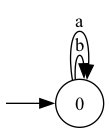
\includegraphics{figures/empty_lang.png}
	\captionsetup{justification=centering}
	\captionsetup{format=hang}
	\singlespace
	\caption{The first DFA generated by L* according to the answers so far, which is the empty language. This DFA is generated before asking the question, is this regex correct? The user then has the chance to view it and provide a counter example.}
	\label{fig:empty_lang}
\end{figure}

\begin{lstlisting}
What is a counter example? abab
Is "ab" in the language? yes
Is "aba" in the language? yes
Is "abab" in the language? yes
Is "aa" in the language? no
Is "abb" in the language? yes
Is "abaa" in the language? yes
Is "ababa" in the language? yes
Is "ababb" in the language? yes
Is "bb" in the language? no
Is "aab" in the language? yes
Is "abbb" in the language? yes
Is "abaab" in the language? yes
Is "ababab" in the language? yes
Is "ababbb" in the language? yes
Is this regex b*aa*b.* correct? yes
\end{lstlisting}

\begin{figure}[H]
\centering
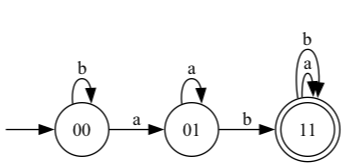
\includegraphics{figures/contains_ab.png}
\captionsetup{justification=centering}
\captionsetup{format=hang}
\singlespace
\caption{This is the second DFA generated by L* according to the current state of the observation table. This DFA does accurately capture that the language contains the string "ab". We accept this proposal and the algorithm concludes the regex \texttt{b*aa*b.*} as the final output.}
\label{fig:contains_ab}
\end{figure}

% \chapter*{\large\bf APPENDIX X: EXAMPLE}
% \addcontentsline{toc}{chapter}{APPENDIX X: EXAMPLE} 

% \renewcommand{\thefigure}{A.\arabic{figure}}
% \setcounter{figure}{0}

% % These two lines reset the counter for tables and adds an "A" before each figure number (i.e, tables A.1)
% \renewcommand{\thetable}{A.\arabic{table}}
% \setcounter{table}{0}

% \renewcommand{\theequation}{A.\arabic{equation}}
% \setcounter{equation}{0}

% \begin{table}[htp]
%     \centering
%     \caption{Call this table A.1.}
%     \label{tab1}
%   	\begin{tabular}{|l|l|l|l|}  % Each "l" corresponds to a column in the table. Hence, the total number of "l"
% 	                            % corresponds to the number of columns your table will have.
% 		\hline
% 		\bf{Heading 1} & \bf{Heading 2} & \bf{Heading 3} & \bf{Heading 4} \\ \hline
% 		Content example. & Content example. & Content example. & Content example. \\ \hline
% 		Content example. & Content example. & Content example. & Content example. \\ \hline
%     \end{tabular}
% \end{table}

% \begin{figure}[H]
% \centering    % This centers it
% 	% \includegraphics[scale=0.10]{figures/blackhole.jpg}
% 	\captionsetup{justification=centering}
% 	\captionsetup{format=hang}
%         \singlespace
% 	\caption{The first recorded image of a black hole}    % This is the caption of the figure
% %\label{figa2}
% \end{figure}

% \begin{equation} \label{Equ.A.1}
% R_{\mu \nu} - {\frac{1}{2}}g_{\mu \nu}\,R + g_{\mu \nu} \Lambda = 
%  {\frac{8 \pi G}{c^4}} T_{\mu \nu}
% \end{equation}
